\documentclass[12pt,twoside]{article}
\usepackage[hmargin=0.8in,vmargin=0.9in]{geometry}
\geometry{letterpaper}
%\usepackage[parfill]{parskip}    % Activate to begin paragraphs with an empty line rather than an indent
%\NeedsTeXFormat{LaTeX2e}
\usepackage{fancyhdr}
\usepackage{graphicx}
%\usepackage{subfigure}
\usepackage{amssymb}
\usepackage{amsmath}
\usepackage{amsfonts}
\usepackage{theorem}
\usepackage{mathrsfs}
\usepackage{mathtools}
\usepackage{bm}
\usepackage{color}
\usepackage{nicefrac}
\usepackage{setspace}
\usepackage{exscale}
\usepackage{relsize}
\usepackage{txfonts}
%\usepackage{doc}
%\usepackage{lastpage}
%\usepackage{longtable}
\usepackage{epstopdf}
\usepackage{float}
%\DeclareGraphicsRule{.tif}{png}{.png}{`convert #1 `dirname #1`/`basename #1 .tif`.png}
\DeclareGraphicsRule{.pstex}{eps}{*}{}
\usepackage{cite}
\usepackage{hyperref}
%\usepackage[numbers,sort&compress]{natbib}
%\usepackage{showkeys}
\usepackage{cleveref}
%\usepackage{refcheck}

\usepackage[absolute,overlay]{textpos}
\usepackage[utf8]{inputenc}
\usepackage[english]{babel}
\usepackage{caption}
\usepackage{subcaption}
\usepackage{pdfpages}
\usepackage{comment}
\usepackage{etoolbox}
\usepackage{tikz}
\usetikzlibrary{calc}

\usepackage{algpseudocode}
\usepackage{algorithm}
\usepackage{multirow}

\usepackage{pgfplots}
\usepackage{pgfplotstable}
\usepackage{stmaryrd}

%\usepackage[noabbrev,capitalise]{cleveref}
%\crefformat{appendix}{#2#1#3}

\usetikzlibrary{fillbetween}
\usepgfplotslibrary{fillbetween}
\usetikzlibrary{shapes.misc}
\usetikzlibrary{math}
\usetikzlibrary{arrows}
\usetikzlibrary{patterns,patterns.meta}


%% LaTeX - Article customise

%%% PACKAGES
%\usepackage{booktabs} % for much better looking tables
\usepackage{array} % for better arrays (eg matrices) in maths
\usepackage{paralist} % very flexible & customisable lists (eg. enumerate/itemize, etc.)
\usepackage{verbatim} % adds environment for commenting out blocks of text & for better verbatim
%\usepackage{subfigure} % make it possible to include more than one captioned figure/table in a single float
% These packages are all incorporated in the memoir class to one degree or another...

%%% HEADERS & FOOTERS
\pagestyle{fancy}
\fancyhead{} % clear all header fields
\fancyhead[LE]{\thepage}
\fancyhead[RO]{\thepage}
\fancyhead[CE]{\sc R. Abgrall, A. Chertock, A. Kurganov \& L. Micalizzi}
\fancyhead[CO]{\sc A New Active Flux Method}
\fancyfoot{} % clear all footer fields
%\fancyfoot[C]{\thepage}
\renewcommand{\headrulewidth}{0.0pt}
\renewcommand{\footrulewidth}{0.0pt}
\addtolength{\headheight}{3pt}
%% END Article customise

\theoremstyle{plain}                    % use "default" font
\newtheorem{thm}{Theorem}[section]
\newtheorem{lemma}[thm]{Lemma}
\newtheorem{proposition}[thm]{Proposition}
\newtheorem{cor}[thm]{Corollary}
\newtheorem{conj}[thm]{Conjecture}
\newtheorem{defn}[thm]{Definition}
\newtheorem{remark}{Remark}[section]
\newenvironment{proof}{{\noindent\it Proof.}\quad}{\hfill $\square$\par}
%{\theorembodyfont{\rmfamily}\newtheorem{remark}{Remark}[section]}
\newenvironment{acknowledgment}{{\flushleft \bf Acknowledgment:}}{}
\newenvironment{DA}{{\flushleft \bf Declarations:}}{}

\renewcommand{\theequation}{\arabic{section}.\arabic{equation}}
\renewcommand{\thefigure}{\arabic{section}.\arabic{figure}}
\renewcommand{\thetable}{\arabic{section}.\arabic{table}}

\renewcommand{\arraystretch}{1.28}
\setlength{\tabcolsep}{1.25mm}

\allowdisplaybreaks[1]

\numberwithin{equation}{section}
\numberwithin{figure}{section}
\numberwithin{table}{section}

\newcommand\eref[1]{(\ref{#1})}
\newcommand{\hilight}[1]{\colorbox{red}{#1}}

\newcommand*\xbar[1]{%
  \hbox{%
    \vbox{%
      \hrule height 0.5pt % The actual bar
      \kern0.4ex%         % Distance between bar and symbol
      \hbox{%
        \kern-0.05em%      % Shortening on the left side
        \ensuremath{#1}%
        \kern-0.00em%      % Shortening on the right side
      }%
    }%
  }%
}

\renewcommand{\arraystretch}{1.3}
\setlength{\tabcolsep}{2.5mm}

\newcommand{\lop}[0]{\mathcal{L}}
\newcommand{\lopd}[0]{\mathcal{L}_\Delta}
\newcommand{\lopdt}[0]{\mathcal{L}_{\Delta}}
\newcommand{\LL}{\lopdt}
\newcommand{\usol}[0]{\underline{\uvec{u}}_\Delta}
\newcommand{\usoldt}[0]{\underline{\uvec{u}}_\Delta}

\newcommand{\up}[0]{\underline{\uvec{u}}^{(p)}}

\newcommand{\usoldto}[0]{\tilde{\underline{\uvec{u}}}_\Delta}

\newcommand{\uapp}[0]{\uvec{u}_h}
\newcommand{\wapp}[0]{w_h}

\newcommand{\massmatrix}[0]{\mathcal{M}}

\newcommand{\tess}[0]{\mathcal{T}_h}


\newcommand{\uvec}[2][3]{\bm{#2\mkern-#1mu}\mkern#1mu}


\newcommand{\res}[0]{\textbf{R}}
\newcommand\norm[1]{\left\lVert#1\right\rVert}
\newcommand\abs[1]{\left\lvert#1\right\rvert}

\newcommand{\flux}[0]{\boldsymbol{F}}
\newcommand{\source}[0]{\boldsymbol{S}}
\newcommand{\ST}[0]{\boldsymbol{ST}_i^K}
\newcommand{\extra}[0]{\boldsymbol{ST}_i}


\newcommand{\elres}[0]{\uvec{\Phi}^K(\uapp)}
\newcommand{\noderes}[0]{\uvec{\Phi}^K_i(\uapp)}
%\newcommand{\spacestuff}[0]{\boldsymbol{\phi}_i}
\newcommand{\cund}[0]{\underline{\uvec{c}}}
\newcommand{\lopdi}[0]{\mathcal{L}_{\Delta,i}}
\newcommand{\csoldt}[0]{\underline{\uvec{c}}_\Delta}
\newcommand{\basis}[0]{\uvec{v}}
\newcommand{\mis}[0]{\mu}
\def\restriction#1#2{\mathchoice
              {\setbox1\hbox{${\displaystyle #1}_{\scriptstyle #2}$}
              \restrictionaux{#1}{#2}}
              {\setbox1\hbox{${\textstyle #1}_{\scriptstyle #2}$}
              \restrictionaux{#1}{#2}}
              {\setbox1\hbox{${\scriptstyle #1}_{\scriptscriptstyle #2}$}
              \restrictionaux{#1}{#2}}
              {\setbox1\hbox{${\scriptscriptstyle #1}_{\scriptscriptstyle #2}$}
              \restrictionaux{#1}{#2}}}
\def\restrictionaux#1#2{{#1\,\smash{\vrule height .8\ht1 depth .85\dp1}}_{\,#2}} 
\newcommand\swapifbranches[3]{#1{#3}{#2}}
\newcommand{\R}{\mathbb{R}}
\newcommand{\redun}[1]{{\color{red} {\large \textit{Is the following redundant?}} #1}}
\newcommand{\davide}[1]{{\color{purple}#1}}
\newcommand{\lore}[1]{ \textbf{{\color{blue}#1}}}
\newcommand{\question}[1]{{\color{red} \large Question: #1 }}
\newcommand{\bbu}{\underline{\uvec{u}}}
\newcommand{\bU}{\uvec{U}}
\newcommand{\bbU}{\underline{\uvec{U}}}
\newcommand{\bbr}{\underline{\uvec{r}}}
\newcommand{\by}{\uvec{y}}
\newcommand{\bby}{\underline{\uvec{y}}}
\newcommand{\bG}{{\uvec{G}}}
\newcommand{\bbt}{\underline{t}}
\newcommand{\vecz}{\underline{0}}
\newcommand{\matz}{\underline{\underline{0}}}
\newcommand{\vecbeta}{\underline{\beta}}
\newcommand{\CIP}{\text{CIP}}
\newcommand{\OSS}{\text{OSS}}
\newcommand{\CFL}{\text{CFL}}

\newcommand{\undu}{\underline{\uvec{u}}}
\newcommand{\undy}{\underline{\uvec{y}}}
\newcommand{\undspacetilde}{\widetilde{\underline{\uvec{\phi}}}}
\newcommand{\spacestuff}{\uvec{\phi}}
\newcommand{\undv}{\underline{\uvec{v}}}
\newcommand{\undw}{\underline{\uvec{w}}}
\newcommand{\undr}{\underline{\uvec{r}}}
\newcommand{\undz}{\underline{\uvec{z}}}
\newcommand{\lopdtp}[0]{\mathcal{L}_{\Delta,p}}
\newcommand{\usolp}[0]{\underline{\uvec{u}}_{\Delta}^{(p)}}
\newcommand{\Xp}[0]{X^{(p)}}
\newcommand{\Yp}[0]{Y^{(p)}}
\newcommand{\uex}[0]{\underline{\uvec{u}}_{ex}}
\newcommand{\uexp}[0]{\underline{\uvec{u}}_{ex}^{(p)}}
\newcommand{\lopdLp}[0]{\mathcal{L}_\Delta^{1,(p)}}
\newcommand{\lopdHp}[0]{\mathcal{L}_\Delta^{2,(p)}}
\newcommand{\embep}[0]{\mathcal{E}^{(p)}}
\newcommand{\projp}[0]{\Pi^{(p)}}
\newcommand{\trialspace}[1]{\varphi_{#1}} %phi space _i
\newcommand{\trialspaceiter}[2]{\varphi_{#1}^{#2}} %phi space _i
\newcommand{\trialtime}[1]{\psi^{#1}} %psi time ^m
\newcommand{\trialtimeiter}[2]{\psi^{#1,#2}} %psi time ^m
%THE FOLLOWING IS  ^l TO AVOID CONFUSION WITH u_n
\newcommand{\trialspacetime}[1]{\vartheta^{#1}} %theta space time 
\newcommand{\trialspacetimeiter}[2]{\vartheta^{#1,#2}}

%ADER-FV
\newcommand{\trialspaceFVp}[1]{\varphi_{#1}} %predictor
\newcommand{\trialspaceFVc}[1]{\lambda_{#1}} %corrector 
\newcommand{\APNPM}{{ADER-$\mathbb P_N \mathbb P_M$ }}

%Temperature
%\newcommand{\Temp}{\tau}
\newcommand{\Temp}{T}


\newcommand{\E}{\boldsymbol{E}}

\newcommand{\pnpm}[2]{\mathbb P_{#1}\mathbb P_{#2}}  %PNPM schemes

\newcommand{\RIcolor}[1]{{\leavevmode\color{black} #1}}
\newcommand{\RIIcolor}[1]{{\leavevmode\color{black} #1}}

\allowdisplaybreaks[1]

\newcommand{\mx}{\bm{x}}
\newcommand{\mpp}{\bm{p}}
\newcommand{\mq}{\bm{q}}
\newcommand{\mf}{\bm{f}}
\newcommand{\mF}{\bm{F}}
\newcommand{\mS}{\bm{S}}
\newcommand{\mg}{\bm{g}}
\newcommand{\mG}{\bm{G}}
\newcommand{\mB}{\bm{B}}
\newcommand{\mC}{\bm{C}}
\newcommand{\mH}{\bm{H}}
\newcommand{\mU}{\bm{U}}
\newcommand{\mV}{\bm{V}}
\newcommand{\mK}{\bm{K}}
\newcommand{\mw}{\bm{w}}
\newcommand{\mW}{\bm{W}}
\newcommand{\mo}{\bm{0}}
\newcommand{\ds}{\displaystyle}
\newcommand{\ovl}{\overline}
\newcommand{\dt}{\Delta t}
\newcommand{\dx}{\Delta x}
\newcommand{\dy}{\Delta y}
\newcommand{\ave}{{\text{ave}}}
\newcommand{\re}{\mathrm{E}}
\newcommand{\rw}{\mathrm{W}}
\newcommand{\rs}{\mathrm{S}}
\newcommand{\rn}{\mathrm{N}}
\newcommand{\rne}{\mathrm{NE}}
\newcommand{\rse}{\mathrm{SE}}
\newcommand{\rnw}{\mathrm{NW}}
\newcommand{\rsw}{\mathrm{SW}}
\newcommand{\hf}{{\frac{1}{2}}}
\newcommand{\hhf}{{\frac{1}{4}}}
\newcommand{\iph}{{i+\frac{1}{2}}}
\newcommand{\imh}{{i-\frac{1}{2}}}
\newcommand{\jph}{{j+\frac{1}{2}}}
\newcommand{\jmh}{{j-\frac{1}{2}}}
\newcommand{\kph}{{k+\frac{1}{2}}}
\newcommand{\kmh}{{k-\frac{1}{2}}}
\newcommand{\lph}{{k+\frac{1}{2}}}
\newcommand{\lmh}{{k-\frac{1}{2}}}
\newcommand{\nmh}{{n-\frac{1}{2}}}

\newcommand{\jlph}{{j_{\ell}+\frac{1}{2}}}
\newcommand{\jlmh}{{j_{\ell}-\frac{1}{2}}}
\newcommand{\jrph}{{j_r+\frac{1}{2}}}
\newcommand{\jrmh}{{j_r-\frac{1}{2}}}
\newcommand{\bh}{\bar{h}}
\newcommand{\bu}{\bar{u}}
\newcommand{\bv}{\bar{v}}
\newcommand{\ves}{\varepsilon}

\newcommand{\B}{\widetilde{B}}
\newcommand{\C}{\widetilde{C}}
\newcommand{\Ubar}{\overline{\uvec{U}}}
\newcommand{\Vbar}{\overline{\uvec{V}}}

\newcommand{\FtildeNum}{\widehat{\widetilde{\uvec{F}}}}
\newcommand{\GtildeNum}{\widehat{\widetilde{\uvec{G}}}}

\newcommand{\Bnonbald}[2]{\widetilde{#1}}
\newcommand{\Bbald}[2]{\widetilde{\uvec{#1}}}

\title{A New Semi-Discrete Finite-Volume Active Flux Method for Hyperbolic Conservation Laws}  
\author{R\'emi Abgrall\thanks{Institute for Mathematics \& Computational Science, University of Zurich, 8057 Zurich, Switzerland;
{\tt remi.abgrall@math.uzh.ch}}, ~Alina Chertock\thanks{Department of Mathematics, North Carolina State University, Raleigh, NC 27695, USA;
{\tt chertock@math.ncsu.edu}}, ~Alexander Kurganov\thanks{Department of Mathematics and Shenzhen International Center for Mathematics,
Southern University of Science and Technology, Shenzhen, 518055, China; {\tt alexander@sustech.edu.cn}},~ and Lorenzo
Micalizzi\thanks{Department of Mathematics, North Carolina State University, Raleigh, NC 27695, USA; {\tt lmicali@ncsu.edu}}}
%\date{\today}
\date{}
\begin{document}
\maketitle
\begin{abstract}
In this work, we introduce a new active flux (AF) method for hyperbolic systems of conservation laws. Following an AF approach recently
proposed in [{\sc R. Abgrall}, Commun. Appl. Math. Comput., 5 (2023), pp. 370--402], we consider two different formulations of the studied
system (the original conservative formulation and a primitive one containing nonconservative products), and discretize them on overlapping
staggered meshes using two different numerical schemes. The novelty of our method is twofold. First, we introduce an original paradigm
making use of overlapping finite-volume (FV) meshes over which cell averages of conservative and primitive variables are evolved using
semi-discrete FV methods: The nonconservative system is discretized by a path-conservative central-upwind scheme and its solution is used to
evaluate very simple numerical fluxes for the discretization of the original conservative system. Second, to ensure the nonlinear stability
of the resulting AF method, we design a post-processing, which also guarantees a conservative coupling between the two sets of variables. We
test the proposed semi-discrete FV AF method on a number of benchmarks for the one- and two-dimensional Euler equations of gas dynamics.
\end{abstract}

\noindent
{\bf Key words:} Active flux methods; overlapping staggered meshes; path-conservative central-upwind schemes; conservative post-processing.
states.

\medskip
\noindent
{\bf AMS subject classification:} 76M12, 65M08, 76N99, 35L65, 35L67.

\section{Introduction}
This paper focuses on the development of numerical methods for hyperbolic systems of conservation laws, which in the two-dimensional (2-D)
case read as
\begin{equation}
\bm U_t+\bm F(\bm U)_x+\bm G(\bm U)_y=\bm0.
\label{1.1}
\end{equation}
Here, $x$ and $y$ are the spatial variables, $t$ is time, $\bm U\in\mathbb R^M$ is the vector of conserved variables,
$\bm F,\bm G\in\mathbb R^M$ are the fluxes, whose Jacobians,
$\frac{\partial\bm F}{\partial\bm U},\frac{\partial\bm G}{\partial\bm U}\in\mathbb R^{M\times M}$, are assumed to be real-diagonalizable,
and $M\in\mathbb N$ with $M\ge1$ is the number of equations in the system.

It is well-known that solutions of nonlinear hyperbolic conservation laws may become nonsmooth even when the initial and boundary data are
infinitely smooth. Therefore, the solution of \eref{1.1} has to be defined in a weak (integral) sense, and hence conservative 
finite-volume (FV) methods seem to be one of the natural choices to be considered. In these methods, the computational domain is covered 
by FV cells and the numerical solution is realized in terms of its cell averages, which are evolved in time using an integral form of 
\eref{1.1}. For a variety of existing FV methods, we refer the reader to \cite{GR3,Hes,LeV02,ToroBook} and references therein.

In this work, we are interested in active flux (AF) methods, which were first introduced in 
\cite{eymann2011active,eymann2013multidimensional} as an extension of the scheme proposed in \cite{van1977towardsiv} for linear hyperbolic 
partial differential equations (PDEs). The key idea of AF methods is to evolve several pieces of information on the computed solution, 
namely, both cell averages and point values at cell interfaces. This gives additional degrees of freedom, which can be used not only to 
enhance the accuracy of the resulting scheme, but also to successfully hybridize conservative and nonconservative numerical methods. As 
demonstrated in \cite{abgrall2010comment}, nonconservative methods cannot be used for accurately solving hyperbolic systems of conservation
laws since nonconservative numerical schemes typically converge to non-entropy  (non-physical) weak solutions. However, in the AF framework,
highly accurate nonconservative methods can be used to evolve the cell interface point values, while the convergence toward the physically
relevant solutions is guaranteed by a conservative evolution of the cell averages. In the past decade, a variety of AF methods have been
developed; see, e.g.,
\cite{Abg23,abgrall2025active,abgrall2023extensions,barsukow2021active,barsukow2019active,chudzik2021cartesian,Roe21,Zeng14}.

A similar idea of obtaining additional degrees of freedom by evolving several pieces of information was used in the methods on overlapping
cells. These methods include both FV \cite{Liu2005,LSTZ2,LSX,XLDLS} and discontinuous Galerkin \cite{LSTZ1,XLDLS,XLS1} ones. In the FV
methods on overlapping cells, hierarchical reconstruction limiters are used to achieve high-order non-oscillatory approximations of the
computed solution, whose cell averages on overlapping cells are evolved in time.
 
In this paper, we incorporate the overlapping FV approach into the AF framework to develop a novel second-order semi-discrete FV AF method.
To this end, we first consider the following nonconservative system, which is equivalent to \eref{1.1} for smooth solutions:
\begin{equation}
\bm V_t+\widetilde{\bm F}(\bm V)_x+\widetilde{\bm G}(\bm V)_y=B(\bm V)\bm V_x+C(\bm V)\bm V_y,
\label{1.2}
\end{equation}
where $\bm V\in\mathbb R^M$ is the vector of primitive variables, $\widetilde{\bm F},\widetilde{\bm G}:\mathbb R^M\to\mathbb R^M$, and
$B,C\in\mathbb R^{M\times M}$. To cite an example, one may consider the Euler equations of gas dynamics, which read as \eref{1.1} with
\begin{equation}
\bm U=(\rho,\rho u,\rho v,E)^\top,~~\bm F(\bm U)=(\rho u,\rho u^2+p,\rho uv,u(E+p))^\top,~~
\bm G(\bm U)=(\rho u,\rho uv,\rho v^2+p,v(E+p))^\top,
\label{1.3f}
\end{equation}
where $\rho$ is the density, $u$ and $v$ are the $x$- and $y$-velocities, $E$ is the total energy, and $p$ is the pressure. We use the
classical closure, obtained with the help of the equation of state of ideal fluids,
\begin{equation}
E=\frac{p}{\gamma-1}+\hf\rho(u^2+v^2),
\label{1.4f}
\end{equation}
in which $\gamma$ is the specific heat ratio. The system \eref{1.1}, \eref{1.3f}--\eref{1.4f} can be rewritten in the nonconservative form
in many different ways, for instance, using the primitive variables $\rho$, $u$, $v$, and $p$, for which the corresponding nonconservative
system reads as \eref{1.2} with
\begin{equation*}
\bm V=(\rho,u,v,p)^\top,\quad\widetilde{\bm F}(\bm V)=\Big(\rho u,\frac{u^2}{2},0,pu\Big)^\top,\quad
\widetilde{\bm G}(\bm V)=\Big(\rho u,0,\frac{v^2}{2},pv\Big)^\top,
\end{equation*}
\begin{equation*}
B^x(\bm V)=\begin{pmatrix}0&0&0&0\\0&0&0&-\frac{1}{\rho}\\0&0&-u&0\\0&-(\gamma-1)p&0&0\end{pmatrix},\quad
B^y(\bm V)=\begin{pmatrix}0&0&0&0\\0&-v&0&0\\0&0&0&-\frac{1}{\rho}\\0&0&-(\gamma-1)p&0\end{pmatrix}.
\end{equation*}

We discretize systems \eref{1.1} and \eref{1.2} on overlapping meshes using a semi-discrete approach, and then solve the resulting systems
of ordinary differential equations (ODEs) simultaneously. The numerical fluxes for the conservative system \eref{1.1} are taken simply as
$\bm F(\bm U(\bm V))$ and $\bm G(\bm U(\bm V))$, while the discretization of the nonconservative system \eref{1.2} is more involved as its
solutions cannot be understood in the sense of distributions. In \cite{dal1995definition}, a concept of Borel measure solutions of
nonconservative systems was introduced (see also \cite{LeF02,LeF}) and later utilized to develop path-conservative numerical methods; see,
e.g., \cite{CLMP,CMP2017,diaz2019path,pares2006numerical,Par2009} and references therein. Here, we discretize \eref{1.2} using a modified
version of the Riemann-problem-solver-free path-conservative central-upwind (PCCU) scheme from \cite{diaz2019path}. The modification is
intended to reduce the amount of numerical dissipation present in the original PCCU scheme and is carried out by replacing the
central-upwind (CU) numerical flux from \cite{kurganov2001semidiscrete}, which was used in \cite{diaz2019path}, with a less dissipative CU
numerical flux from \cite{KLin}.

Since the conservative numerical fluxes do not employ any limiting procedures, one can expect the computed $\bm U$ to be oscillatory. At 
At the same time, variables $\bm V$, computed in a non-oscillatory manner by the PCCU scheme, may converge to a non-physical weak solution.
We therefore introduce a conservative post-processing, which couples the evolution of the two sets of variables. The resulting numerical
solution is (essentially) oscillation-free and the scheme converges to the physically relevant solution of \eref{1.1}. We test the proposed
FV AF method on a number of benchmarks for one- and two-dimensional Euler equations of gas dynamics.

The rest of the paper is organized as follows. In \S\ref{sec2}, we introduce the new one-dimensional (1-D) FV AF method, and then extend 
it to the 2-D case in \S\ref{sec3}. In \S\ref{sec4}, we report the results of several numerical experiments for both 1-D and 2-D Euler
equations of gas dynamics. Finally, in \S\ref{sec5}, we provide concluding remarks and discuss future perspectives.

\section{One-Dimensional Semi-Discrete FV AF Method}\label{sec2}
In this section, we introduce the new semi-discrete FV AF method for the 1-D version of \eref{1.1}:
\begin{equation}
\bm U_t+\bm F(\bm U)_x=\bm0,
\label{2.1}
\end{equation}
whose nonconservative formulation reads as
\begin{equation}
\bm V_t+\widetilde{\bm F}(\bm V)_x=B(\bm V)\bm V_x.
\label{2.2}
\end{equation}

We consider overlapping FV meshes consisting of uniform cells $I_j=[x_\jmh,x_\jph]$, $j=1,\ldots,N$ and $I_\jph=[x_j,x_{j+1}]$,
$j=0,\ldots,N$ with $x_{j+1}=x_\jph+\dx/2=x_j+\dx$ for all $j$. As in all FV methods, the computed quantities are cell averages of $\bm U$
and $\bm V$, which are obtained on the above two grids, namely,
$$
\xbar{\bm U}_j:\approx\int\limits_{I_j}\bm U(x,t)\,{\rm d}x\quad\mbox{and}\quad
\xbar{\bm V}_\jph:\approx\int\limits_{I_\jph}\bm V(x,t)\,{\rm d}x.
$$
Note that both $\xbar{\bm U}_j$ and $\xbar{\bm V}_\jph$, like many other indexed quantities below, depend on time, but we omit this
dependence for the sake of notation brevity.

The semi-discretization of the conservative system \eref{2.1} is obtained by integrating \eref{2.1} in space over the cells $I_j$, which
results in
\begin{equation}
\frac{\rm d}{{\rm d}t}\,\xbar{\bm U}_j=-\frac{1}{\dx}\Big[\bm{{\cal F}}_\jph-\bm{{\cal F}}_\jmh\Big],
\label{2.3}
\end{equation}
in which we take the following simple numerical fluxes:
\begin{equation}
\bm{{\cal F}}_\jph=\bm F\big(\bm U_\jph\big),\quad\bm U_\jph:=\bm U\big(\,\xbar{\bm V}_\jph\big),
\label{2.4}
\end{equation}
where $\bm U(\bm V)$ denotes the transformation from primitive to conserved variables. Note that for second-order methods, cell averages and
point values formally differ by ${\cal O}((\dx)^2)$, which makes the transformation used in \eref{2.4} straightforward, while higher order
extensions would require a suitable higher order reconstruction of point values.

The semi-discretization of the nonconservative system \eref{2.2} is obtained through the modified PCCU scheme and reads
\begin{equation}
\frac{\rm d}{{\rm d}t}\Vbar_\jph=-\frac{1}{\dx}\bigg[\widetilde{\bm{{\cal F}}}_{j+1}-\widetilde{\bm{{\cal F}}}_j-\bm B_\jph
-\frac{a^+_j}{a^+_j-a^-_j}\bm B_{\bm\Psi,j}+\frac{a^-_{j+1}}{a^+_{j+1}-a^-_{j+1}}\bm B_{\bm\Psi,j+1}\bigg],
\label{2.5}
\end{equation}
where $\widetilde{\bm{{\cal F}}}_j$ are the CU numerical fluxes from \cite{KLin} given by
\begin{equation}
\widetilde{\bm{{\cal F}}}_j=\frac{a^+_j\widetilde{\bm F}\big(\bm V^-_j\big)-a^-_j\widetilde{\bm F}\big(\bm V^+_j\big)}{a^+_j-a^-_j}+
\frac{a^+_ja^-_j}{a^+_j-a^-_j}\Big(\bm V^+_j-\bm V^-_j-\delta\bm V_j\Big).
\label{2.6}
\end{equation}
Here, $\bm V^\pm_j$ are one-sided point values of $\bm V$ obtained using a piecewise linear reconstruction applied to the local
characteristic variables $\bm\Gamma$ of\eref{1.2}. To this end, we follow \cite{micalizzitoro2024} and introduce
$$
\bm\Gamma_\jmh=Q_\jph^{-1}\xbar{\bm V}_\jmh,\quad\bm\Gamma_\jph=Q_\jph^{-1}\xbar{\bm V}_\jph,\quad
\bm\Gamma_{j+\frac{3}{2}}=Q_\jph^{-1}\xbar{\bm V}_{j+\frac{3}{2}},
$$
where $Q_\jph$ is a matrix such that $Q_\jph^{-1}{\cal A}_\jph Q_\jph$ is a diagonal matrix and
${\cal A}_\jph={\cal A}\big(\xbar{\bm V}_\jph\big):=\frac{\partial\widetilde{\bm F}}{\partial\bm V}\big(\xbar{\bm V}_\jph\big)-
B\big(\xbar{\bm V}_\jph\big)$. Equipped with $\bm\Gamma_\jmh$, $\bm\Gamma_\jph$, and $\bm\Gamma_{j+\frac{3}{2}}$, we apply a generalized
minmod limiter (see, e.g., \cite{LN,sweby1984high}) to evaluate
$$
(\bm\Gamma_x)_\jph={\rm minmod}\left(\theta\,\frac{\bm\Gamma_\jph-\bm\Gamma_\jmh}{\dx},
\frac{\bm\Gamma_{j+\frac{3}{2}}-\bm\Gamma_\jmh}{2\dx},\,\theta\,\frac{\bm\Gamma_{j+\frac{3}{2}}-\bm\Gamma_\jph}{\dx}\right),\quad
\theta\in[1,2],
$$
where the minmod function, defined as
\begin{equation*}
{\rm minmod}(c_1,c_2,\ldots)=
\left\{\begin{aligned}
&\min_ic_i&&\mbox{if}~c_i>0~~\forall i,\\
&\max_ic_i&&\mbox{if}~c_i<0~~\forall i,\\
&0&&\mbox{otherwise},
\end{aligned}\right.
\end{equation*}
is applied in a component-wise manner. We then obtain
$$
\bm\Gamma_j^+=\bm\Gamma_\jph-\frac{\dx}{2}(\bm\Gamma_x)_\jph,\quad\bm\Gamma_{j+1}^-=\bm\Gamma_\jph+\frac{\dx}{2}(\bm\Gamma_x)_\jph\textcolor{red}{,}
$$
and hence the corresponding point values of $\bm V$ are
$$
\bm V^+_j=Q_\jph\bm\Gamma_j^+,\quad\bm V^-_{j+1}=Q_\jph\bm\Gamma_{j+1}^-.
$$
In \eref{2.5} and \eref{2.6}, $a^\pm_j$ are the one-sided local speeds of propagation, which can be estimated by
\begin{equation*}
a^-_j=\min\left\{\lambda_1(\bm V^-_j),\lambda_1(\bm V^+_j),0\right\},\quad
a^+_j=\max\left\{\lambda_M(\bm V^-_j),\lambda_M(\bm V^+_j),0\right\}.
\end{equation*}
where $\lambda_1(\bm V)\le\ldots\le\lambda_M(\bm V)$ are the eigenvalues of ${\cal A}(\bm V)$. The term $\delta\bm V_j$ in \eref{2.6}
represents ``built-in'' anti-diffusion and is given by (see \cite{KLin}),
\begin{equation*}
\delta\bm V_j={\rm minmod}\left(\bm V_j^*-\bm V^-_j,\bm V^+_j-\bm V_j^*\right),\quad
\bm V_j^*:=\frac{a^+_j\bm V^+_j-a^-_j\bm V^-_j-\widetilde{\bm F}(\bm V^+_j)+\widetilde{\bm F}(\bm V^-_j)}{a^+_j-a^-_j}.
\end{equation*}
Finally, the terms $\bm B_\jph$ and $\bm B_{\bm\Psi,j}$ in \eref{2.5} are given by (see \cite{diaz2019path} for details)
\begin{equation*}
\bm B_\jph=B\big(\xbar{\bm V}_\jph\big)\big(\bm V_{j+1}^--\bm V_j^+\big),\quad
\bm B_{\bm\Psi,j}=\hf\left[B(\bm V_j^-)+B\big(\bm V_j^+\big)\right]\big(\bm V_j^+-\bm V_j^-\big).
\end{equation*}
\begin{remark}
We would like to stress that the proposed FV AF method is not tied to the PCCU scheme and, in principle, one can numerically solve the
nonconservative system \eref{2.2} using an alternative second-order stable numerical method instead.
\end{remark}

The ODE systems \eref{2.3} and \eref{2.5} should be numerically solved by a stable and sufficiently accurate ODE solver. However, the
solution obtained upon completion of a time step evolution will have two significant drawbacks. First, the solution realized by
$\big\{\,\xbar{\bm U}_j(t+\dt)\big\}$ will likely be oscillatory since no limiting procedures are employed in the computation of numerical
fluxes in \eref{2.4}. Second, the solution realized by $\big\{\xbar{\bm V}_\jph(t+\dt)\big\}$ will not necessarily be conservative, that 
is, $\sum_j\bm U\big(\xbar{\bm V}_\jph(t+\dt)\big)$ may not be equal to $\sum_j\bm U\big(\xbar{\bm V}_\jph(t)\big)$. Therefore, to
ensure that the resulting numerical solution is (essentially) oscillation-free and converges to the physically relevant solution of
\eref{2.1}, we propose the conservative post-processing procedure presented in the next subsection.

\subsection{Post-Processing}
Let us assume that the solution was evolved from time $t$ to $t+\dt$ with the help of an ODE solver and denote the obtained solutions by
$\big\{\,\xbar{\bm U}_j^{\,*}\big\}$ and $\big\{\xbar{\bm V}_\jph^{\,*}\big\}$. Our goal is to modify these values through a suitable
post-processing procedure to obtain non-oscillatory sets of $\big\{\,\xbar{\bm U}_j(t+\dt)\big\}$ and
$\big\{\xbar{\bm V}_\jph(t+\dt)\big\}$.

The proposed post-processing can be presented algorithmically through the following four steps.

\vskip3pt
\noindent
{\bf Step 1.} Compute the conserved variables at $x=x_\jph$ using the transformation from the primitive ones:
$$
\bm U_\jph^*:=\bm U\big(\xbar{\bm V}_\jph^{\,*}\big).
$$

\vskip3pt
\noindent
{\bf Step 2.} Perform the piecewise linear reconstruction for $\bm U$ using the slopes computed by the minmod limiter
$$
(\bm U_x)_j^*=2\,{\rm minmod}\left(\frac{\,\xbar{\bm U}_j^{\,*}-\bm U_\jmh^*}{\dx},\frac{\bm U_\jph^*-\,\xbar{\bm U}_j^{\,*}}{\dx}\right),
$$
which results in
\begin{equation}
\bm U_\jph^{*,-}:=\,\xbar{\bm U}_j^{\,*}+\frac{\dx}{2}(\bm U_x)_j^*,\quad
\bm U_\jph^{*,+}:=\,\xbar{\bm U}_{j+1}^{\,*}-\frac{\dx}{2}(\bm U_x)_{j+1}^*.
\label{2.7}
\end{equation}

\vskip3pt
\noindent
{\bf Step 3.} Set
\begin{equation}
\bm U_\jph^{**}:=\hf\Big(\bm U_\jph^{*,-}+\bm U_\jph^{*,+}\Big),
\label{2.8}
\end{equation}
and recompute the primitive variables at $x=x_\jph$ using the transformation from the conservative ones:
$$
\xbar{\bm V}_\jph(t+\dt)=\bm V\big(\bm U_\jph^{**}\big).
$$

\vskip3pt
\noindent
{\bf Step 4.} Correct the conserved variables by setting
\begin{equation}
\xbar{\bm U}_j(t+\dt)=\hf\Big(\bm U_\jmh^{**}+\bm U_\jph^{**}\Big).
\label{2.9}
\end{equation}

\vskip7pt
It is important to stress that the post-processing is conservative as shown in the next proposition.
\begin{proposition}
The post-processed cell averages of the conserved variables satisfy
\begin{equation*}
\sum_j\,\xbar{\bm U}_j(t+\dt)=\sum_j\,\xbar{\bm U}_j^{\,*}.
\end{equation*}
\end{proposition}
\begin{proof}
The proof consists of simple direct computations (assuming no contributions from the boundary terms):
$$
\begin{aligned}
\sum_j\,\xbar{\bm U}_j(t+\dt)&\stackrel{\eref{2.9}}{=}\hf\sum_j\bm U_\jmh^{**}+\hf\sum_j\bm U_\jph^{**}=\sum_j\bm U_\jph^{**}
\stackrel{\eref{2.8}}{=}\hf\sum_j\bm U_\jph^{*,-}+\hf\sum_j\bm U_\jph^{*,+}\\
&\stackrel{\eref{2.7}}{=}\hf\sum_j\Big[\,\xbar{\bm U}_j^{\,*}+\frac{\dx}{2}(\bm U_x)_j^*\Big]+
\hf\sum_j\Big[\,\xbar{\bm U}_{j+1}^{\,*}-\frac{\dx}{2}(\bm U_x)_{j+1}^*\Big]=\sum_j\,\xbar{\bm U}_j^{\,*}.
\end{aligned}
$$
\end{proof}

\section{Two-Dimensional Semi-Discrete FV AF Method}\label{sec3}
We now extend the proposed semi-discrete FV AF method to the 2-D case, in which the conservative and nonconservative (primitive)
formulations of the governing equations are given by \eref{1.1} and \eref{1.2}, respectively. 

We consider overlapping Cartesian meshes (see the sketch in Figure \ref{fig31}) consisting of uniform cells
$I_{j,k}:=[x_\jmh,x_\jph]\times[y_\kmh,y_\kph]$, $j=1,\ldots,N_x$, $k=1,\ldots,N_y$, $I_{\jph,k}^x=[x_j,x_{j+1}]\times[y_\kmh,y_\kph]$,
$j=0,\ldots,N_x$, $k=1,\ldots,N_y$, and $I_{j,\kph}^y=[x_\jmh,x_\jph]\times[y_k,y_{k+1}]$, $j=1,\ldots,N_x$, $k=0,\ldots,N_y$ with
$x_{j+1}=x_\jph+\dx/2=x_j+\dx$ for all $j$ and $y_{k+1}=y_\kph+\dy/2=y_k+\dy$ for all $k$. The computed quantities are the following cell
averages obtained on the above three grids:
$$
\xbar{\bm U}_{j,k}:\approx\int\limits_{I_{j,k}}\bm U(x,t)\,{\rm d}x{\rm d}y,\quad
\xbar{\bm V}^{\,x}_{\jph,k}:\approx\int\limits_{I_{\jph,k}^x}\bm V(x,t)\,{\rm d}x{\rm d}y,\quad
\xbar{\bm V}^{\,y}_{j,\kph}:\approx\int\limits_{I_{j,\kph}^y}\bm V(x,t)\,{\rm d}x{\rm d}y.
$$
\begin{figure}[ht!]
\vskip-40pt
\centering
\scalebox{0.9}{
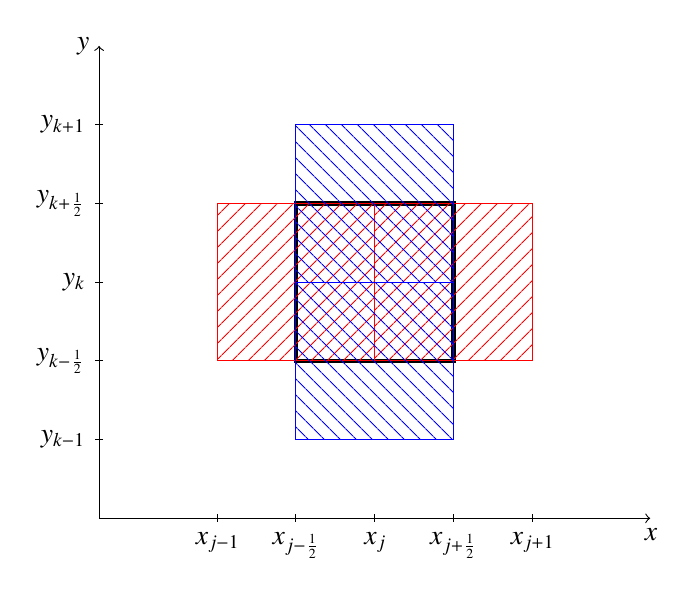
\begin{tikzpicture}
\def\s{2}
% Shifted Cartesian axes outside the picture
\begin{scope}[shift={(-0.5,0)}]  % Adjust shift to move axes away
\draw[->] (0,0) -- (7,0) node[below] {$x$};
\draw[->] (0,0) -- (0,6) node[left] {$y$};
% x-axis labels
\foreach\x/\lab in {1.5/{$x_{j-1}$},2.5/{$x_\jmh$},3.5/{$x_j$},4.5/{$x_\jph$},5.5/{$x_{j+1}$}}{\draw (\x,0.05) -- (\x,-0.05);
\node[below] at (\x,-0.05){\lab};}
% y-axis labels
\foreach \y/\lab in {1/{$y_{k-1}$},2/{$y_\kmh$},3/{$y_k$},4/{$y_\kph$},5/{$y_{k+1}$}}{\draw (0.05,\y) -- (-0.05,\y);
\node[left] at (-0.05,\y){\lab};}
\end{scope}
% Central black square with no fill
\draw[ultra thick] (\s,\s) rectangle (2*\s,2*\s);
% Red staggered squares (filled with /// pattern)
\fill[pattern={Lines[angle=45, distance=4pt, line width=0.4pt]}, pattern color=red] (0.5*\s,\s) rectangle (1.5*\s,2*\s);
\draw[red] (0.5*\s,\s) rectangle (1.5*\s,2*\s);
\fill[pattern={Lines[angle=45, distance=4pt, line width=0.4pt]}, pattern color=red] (1.5*\s,\s) rectangle (2.5*\s,2*\s);
\draw[red] (1.5*\s,\s) rectangle (2.5*\s,2*\s);
% Blue staggered squares (filled with \\\ pattern)
\fill[pattern={Lines[angle=135, distance=4pt, line width=0.4pt]}, pattern color=blue] (\s,0.5*\s) rectangle (2*\s,1.5*\s);
\draw[blue] (\s,0.5*\s) rectangle (2*\s,1.5*\s);
\draw[blue] (\s,0.5*\s) rectangle (2*\s,1.5*\s);
\fill[pattern={Lines[angle=135, distance=4pt, line width=0.4pt]}, pattern color=blue] (\s,1.5*\s) rectangle (2*\s,2.5*\s);
\draw[blue] (\s,1.5*\s) rectangle (2*\s,2.5*\s);
\end{tikzpicture}}
\caption{\sf Sketch of the overlapping cells: $I_{j,k}$ (black-bordered); $I_{\jmh,k}^x$ and $I_{\jph,k}^X$ (red-filled); $I_{j,\kmh}^y$
and $I_{j,\kph}^y$ (blue-filled).
\label{fig31}}
\end{figure}

As in the 1-D case, the semi-discretization of the conservative system \eref{1.1} is obtained by integrating \eref{1.1} in space over the
cells $I_{j,k}$, which leads to
\begin{equation*}
\frac{\rm d}{{\rm d}t}\,\xbar{\bm U}_{j,k}=-\frac{1}{\dx}\Big[\bm{{\cal F}}_{\jph,k}-\bm{{\cal F}}_{\jmh,k}\Big]-
\frac{1}{\dy}\Big[\bm{{\cal G}}_{j,\kph}-\bm{{\cal G}}_{j,\kmh}\Big],
\end{equation*}
with the following second-order numerical fluxes:
$$
\bm{{\cal F}}_{\jph,k}=\bm F\big(\bm U_{\jph,k}\big),~~\bm U_{\jph,k}:=\bm U\big(\,\xbar{\bm V}^{\,x}_{\jph,k}\big)\quad\mbox{and}\quad
\bm{{\cal G}}_{j,\kph}=\bm G\big(\bm U_{j,\kph}\big),~~\bm U_{j,\kph}:=\bm U\big(\,\xbar{\bm V}^{\,y}_{j,\kph}\big).
$$

Two {\em independent} semi-discretizations of the nonconservative system \eref{1.2} are obtained through the modified 2-D PCCU scheme
applied on the $I_{\jph,k}^x$ and $I_{j,\kph}^y$ meshes, respectively, as follows:
\allowdisplaybreaks
\begin{align}
&\begin{aligned}
\frac{\rm d}{{\rm d}t}\,\xbar{\bm V}^{\,x}_{\jph,k}=&-\frac{1}{\dx}\bigg[\widetilde{\bm{{\cal F}}}^{\,x}_{j+1,k}-
\widetilde{\bm{{\cal F}}}^{\,x}_{j,k}-\bm B^x_{\jph,k}-\frac{a^{x,+}_{j,k}}{a^{x,+}_{j,k}-a^{x,-}_{j,k}}\,\bm B^x_{\bm\Psi,j,k}+
\frac{a^{x,-}_{j+1,k}}{a^{x,+}_{j+1,k}-a^{x,-}_{j+1,k}}\,\bm B^x_{\bm\Psi,j+1,k}\bigg]\\
&-\frac{1}{\dy}\bigg[\widetilde{\bm{{\cal G}}}^{\,x}_{\jph,\kph}-\widetilde{\bm{{\cal G}}}^{\,x}_{\jph,\kmh}-\bm C^x_{\jph,k}\\
&\hspace{1.6cm}-\frac{b^{x,+}_{\jph,\kmh}}{b^{x,+}_{\jph,\kmh}-b^{x,-}_{\jph,\kmh}}\,\bm C^x_{\bm\Psi,\jph,\kmh}+
\frac{b^{x,-}_{\jph,\kph}}{b^{x,+}_{\jph,\kph}-b^{x,-}_{\jph,\kph}}\,\bm C^x_{\bm\Psi,\jph,\kph}\bigg]
\end{aligned}
\label{3.1}\\
&\begin{aligned}
\frac{\rm d}{{\rm d}t}\,\xbar{\bm V}^{\,y}_{j,\kph}=&-\frac{1}{\dx}\bigg[\widetilde{\bm{{\cal F}}}^{\,y}_{\jph,\kph}-
\widetilde{\bm{{\cal F}}}^{\,y}_{\jmh,\kph}-\bm B^y_{j,\kph}\\
&\hspace{1.25cm}-\frac{a^{y,+}_{\jmh,\kph}}{a^{y,+}_{\jmh,\kph}-a^{y,-}_{\jmh,\kph}}\,\bm B_{\bm\Psi,\jmh,\kph}^y+
\frac{a^{y,-}_{\jph,\kph}}{a^{y,+}_{\jph,\kph}-a^{y,-}_{\jph,\kph}}\,\bm B^y_{\bm\Psi,\jph,\kph}\bigg]\\
&-\frac{1}{\dy}\bigg[\widetilde{\bm{{\cal G}}}^{\,y}_{j,k+1}-\widetilde{\bm{{\cal G}}}^{\,y}_{j,k}-\bm C^y_{j,\kph}
-\frac{b^{y,+}_{j,k}}{b^{y,+}_{j,k}-b^{y,-}_{j,k}}\,\bm C^y_{\bm\Psi,j,k}+
\frac{b^{y,-}_{j,k+1}}{b^{y,+}_{j,k+1}-b^{y,-}_{j,k+1}}\,\bm C^y_{\bm\Psi,j,k+1}\bigg]
\end{aligned}
\label{3.2}
\end{align}
Once again, we stress that the right-hand sides (RHSs) of \eref{3.1} and \eref{3.2} are computed independently and thus their computations
can be performed in parallel.

The terms on the RHS of \eref{3.1} are computed in a dimension-by-dimension manner and given by
\allowdisplaybreaks
\begin{align*}
&\widetilde{\bm{{\cal F}}}^{\,x}_{j,k}=\frac{a^{x,+}_{j,k}\widetilde{\bm F}\big(\bm V^{x,-}_{j,k}\big)-
a^{x,-}_{j,k}\widetilde{\bm F}\big(\bm V^{x,+}_{j,k}\big)}{a^{x,+}_{j,k}-a^{x,-}_{j,k}}+
\frac{a^{x,+}_{j,k}a^{x,-}_{j,k}}{a^{x,+}_{j,k}-a^{x,-}_{j,k}a\,}\Big(\bm V^{x,+}_{j,k}-\bm V^{x,-}_{j,k}-\delta\bm V^x_{j,k}\Big),\\
&\delta\bm V^x_{j,k}={\rm minmod}\left(\bm V_{j,k}^{x,*}-\bm V^{x,-}_{j,k},\bm V^{x,+}_{j,k}-\bm V_{j,k}^{x,*}\right),\quad
\bm V_{j,k}^{x,*}=\frac{a^{x,+}_{j,k}\bm V^{x,+}_{j,k}-a^{x,-}_{j,k}\bm V^{x,-}_{j,k}-\widetilde{\bm F}(\bm V^{x,+}_{j,k})+
\widetilde{\bm F}(\bm V^{x,-}_{j,k})}{a^{x,+}_{j,k}-a^{x,-}_{j,k}},\\
&\widetilde{\bm{{\cal G}}}^x_{\jph,\kph}=\frac{b^{x,+}_{\jph,\kph}\widetilde{\bm G}\big(\bm V^{x,-}_{\jph,\kph}\big)-
b^{x,-}_{\jph,\kph}\widetilde{\bm G}\big(\bm V^{x,+}_{\jph,\kph}\big)}{b^{x,+}_{\jph,\kph}-b^{x,-}_{\jph,\kph}}\\
&\hspace{1.4cm}+\frac{b^{x,+}_{\jph,\kph}b^{x,-}_{\jph,\kph}}{b^{x,+}_{\jph,\kph}-b^{x,-}_{\jph,\kph}}\,
\Big(\bm V^{x,+}_{\jph,\kph}-\bm V^{x,-}_{\jph,\kph}-\delta\bm V^x_{\jph,\kph}\Big),\\
&\delta\bm V^x_{\jph,\kph}={\rm minmod}\Big(\bm V_{\jph,\kph}^{x,*}-\bm V^{x,-}_{\jph,\kph},
\bm V^{x,+}_{\jph,\kph}-\bm V_{\jph,\kph}^{x,*}\Big),\\
&\bm V_{\jph,\kph}^{x,*}=\frac{b^{x,+}_{\jph,\kph}\bm V^{x,+}_{\jph,\kph}-b^{x,-}_{\jph,\kph}\bm V^{x,-}_{\jph,\kph}-
\widetilde{\bm G}\big(\bm V^{x,+}_{\jph,\kph}\big)+\widetilde{\bm G}\big(\bm V^{x,-}_{\jph,\kph}\big)}
{b^{x,+}_{\jph,\kph}-b^{x,-}_{\jph,\kph}},\\
&\bm B^x_{\jph,k}=B\big(\xbar{\bm V}^x_{\jph,k}\big)\big(\bm V_{j+1,k}^{x,-}-\bm V_{j,k}^{x,+}\big),\quad
\bm B^x_{\bm\Psi,\jph,k}=\hf\Big[B(\bm V_{\jph,k}^{x,-})+B\big(\bm V_{\jph,k}^{x,+}\big)\Big]
\big(\bm V_{\jph,k}^{x,+}-\bm V_{\jph,k}^{x,-}\big),\\
&C^x_{\jph,k}=C\big(\xbar{\bm V}^x_{\jph,k}\big)\big(\bm V_{\jph,\kph}^{x,-}-\bm V_{\jph,\kmh}^{x,+}\big),\\
&\bm C^x_{\bm\Psi,\jph,\kph}=\hf\Big[C(\bm V_{\jph,\kph}^{x,-})+C\big(\bm V_{\jph,\kph}^{x,+}\big)\Big]
\big(\bm V_{\jph,\kph}^{x,+}-\bm V_{\jph,\kph}^{x,-}\big),
\end{align*}
where $\bm V^{x,\pm}_{j,k}$ and $\bm V^{x,\pm}_{\jph,\kph}$ are reconstructed point values obtained from the cell averages
$\big\{\xbar{\bm V}^{\,x}_{j,k}\big\}$. As in the 1-D case, we compute these values by exploiting the local characteristic decomposition. 
In the $x$-direction, we have
$$
\bm V^{x,+}_{j,k}=Q^x_{\jph,k}\bm\Gamma_{j,k}^{x,+},\quad\bm V^{x,-}_{j+1,k}=Q^x_{\jph,k}\bm\Gamma_{j+1,k}^{x,-},
$$
where
$$
\bm\Gamma_{j,k}^{x,+}=\bm\Gamma^x_{\jph,k}-\frac{\dx}{2}(\bm\Gamma_x)^x_{\jph,k},\quad
\bm\Gamma_{j+1,k}^{x,-}=\bm\Gamma^x_{\jph,k}+\frac{\dx}{2}(\bm\Gamma_x)^x_{\jph,k}
$$
with the slopes computed using the generalized minmod limiter:
\begin{equation}
(\bm\Gamma_x)^x_{\jph,k}={\rm minmod}\left(\theta\,\frac{\bm\Gamma^x_{\jph,k}-\bm\Gamma^x_{\jmh,k}}{\dx},
\frac{\bm\Gamma^x_{j+\frac{3}{2},k}-\bm\Gamma^x_{\jmh,k}}{2\dx},
\,\theta\,\frac{\bm\Gamma^x_{j+\frac{3}{2},k}-\bm\Gamma^x_{\jph,k}}{\dx}\right),\quad\theta\in[0,1].
\label{3.3}
\end{equation}
In \eref{3.3}, one has
$$
\bm\Gamma^x_{\jmh,k}=\big(Q^x_{\jph,k}\big)^{-1}\,\xbar{\bm V}^{\,x}_{\jmh,k},\quad
\bm\Gamma^x_{\jph,k}=\big(Q_{\jph,k}^x\big)^{-1}\,\xbar{\bm V}^{\,x}_{\jph,k},\quad
\bm\Gamma^x_{j+\frac{3}{2},k}=\big(Q_{\jph,k}^x\big)^{-1}\,\xbar{\bm V}^{\,x}_{j+\frac{3}{2},k},
$$
where the matrix $Q^x_{\jph,k}$ is such that $\big(Q^x_{\jph,k}\big)^{-1}{\cal A}^x_{\jph,k}Q^x_{\jph,k}$ is diagonal with
${\cal A}^x_{\jph,k}={\cal A}\big(\xbar{\bm V}^{\,x}_{\jph,k}\big):=
\frac{\partial\widetilde{\bm F}}{\partial\bm V}\big(\xbar{\bm V}^{\,x}_{\jph,k}\big)-B\big(\xbar{\bm V}^{\,x}_{\jph,k}\big)$. 

Similarly, in the $y$-direction, we have
$$
\bm V^{x,+}_{\jph,\kmh}=P^x_{\jph,k}\bm\Gamma_{\jph,\kmh}^{x,+},\quad\bm V^{x,-}_{\jph,\kph}=P^x_{\jph,k}\bm\Gamma_{\jph,\kph}^{x,-},
$$
where
$$
\bm\Gamma_{\jph,\kmh}^{x,+}=\bm\Gamma^x_{\jph,k}-\frac{\dy}{2}(\bm\Gamma_y)^x_{\jph,k},
\quad\bm\Gamma_{\jph,k}^{x,-}=\bm\Gamma_{\jph,k}^x+\frac{\dy}{2}(\bm\Gamma_y)^x_{\jph,k}
$$
with the slope given by
\begin{equation}
(\bm\Gamma_y)^x_{\jph,k}={\rm minmod}\left(\theta\,\frac{\bm\Gamma^x_{\jph,k}-\bm\Gamma^x_{\jph,k-1}}{\dy},
\frac{\bm\Gamma^x_{\jph,k+1}-\bm\Gamma^x_{\jph,k-1}}{2\dy},\,\theta\,\frac{\bm\Gamma^x_{\jph,k+1}-\bm\Gamma^x_{\jph,k}}{\dy}\right),\quad
\theta\in[0,1].
\label{3.4}
\end{equation}
In \eref{3.4}, one has
$$
\bm\Gamma^x_{\jph,k-1}=(P_{\jph,k}^x)^{-1}\xbar{\bm V}^{\,x}_{\jph,k-1},\quad
\bm\Gamma^x_{\jph,k}=(P^x_{\jph,k})^{-1}\xbar{\bm V}^{\,x}_{\jph,k},\quad
\bm\Gamma^x_{\jph,k+1}=(P_{\jph,k}^x)^{-1}\xbar{\bm V}^{\,x}_{\jph,k+1},
$$
where the matrix $P^x_{\jph,k}$ is such that $(P^x_{\jph,k})^{-1}{\cal B}^x_{\jph,k} P^x_{\jph,k}$ is diagonal with
${\cal B}^x_{\jph,k}={\cal B}\big(\xbar{\bm V}_{\jph,k}^{\,x}\big):=
\frac{\partial\widetilde{\bm G}}{\partial\bm V}\big(\xbar{\bm V}^{\,x}_{\jph,k}\big)-C\big(\xbar{\bm V}^{\,x}_{\jph,k}\big)$. 

The one-sided local speeds of propagation in \eref{3.1} are estimated by
\begin{equation*}
\begin{aligned}
&a^{x,-}_{j,k}=\min\left\{\lambda_1(\bm V^{x,-}_{j,k}),\lambda_1(\bm V^{x,+}_{j,k}),0\right\},&&
a^{x,+}_{j,k}=\max\left\{\lambda_M(\bm V^{x,-}_{j,k}),\lambda_M(\bm V^{x,+}_{j,k}),0\right\},\\
&b^{x,-}_{\jph,\kph}=\min\left\{\mu_1(\bm V^{x,-}_{\jph,\kph}),\mu_1(\bm V^{x,+}_{\jph,\kph}),0\right\},&&
b^{x,+}_{\jph,\kph}=\max\left\{\mu_M(\bm V^{x,-}_{\jph,\kph}),\mu_M(\bm V^{x,+}_{\jph,\kph}),0\right\},
\end{aligned}
\end{equation*}
where $\lambda_1(\bm V)\le\ldots\le\lambda_M(\bm V)$ are the eigenvalues of ${\cal A}(\bm V)$ and
$\mu_1(\bm V)\le\ldots\le\mu_M(\bm V)$ are the eigenvalues of ${\cal B}(\bm V)$. 

The terms on the RHS of \eref{3.2}, related to the update of $\xbar{\bm V}^{\,y}_{j,\kph}$, can be analogously computed through the same
formulae used to evaluate the RHS of \eref{3.1}, but with the first index shifted by $-\hf$, the second index shifted by $+\hf$, and the
superscripts ``$x$'' replaced by ``$y$''.
\begin{remark}
We would like to emphasize that, as in the 1-D case, the proposed 2-D FV AF method is not tied to the PCCU scheme and the nonconservative
system \eref{1.2} can be numerically solved by an alternative second-order stable numerical method.
\end{remark}

Finally, the post-processing is carried out in a ``dimension-by-dimension'' manner by alternating sweeps in the $x$-direction, in which we
modify the cell averages of $\xbar{\bm U}$ and $\xbar{\bm V}^{\,x}$, and in the $y$-direction, in which we modify the cell averages of
$\xbar{\bm U}$ and $\xbar{\bm V}^{\,y}$. We use the same notation as in the 1-D case: $\big\{\,\xbar{\bm U}_{j,k}^{\,*}\big\}$, 
$\big\{\xbar{\bm V}_{\jph,k}^{\,x,*}\big\}$, and $\big\{\xbar{\bm V}_{j,\kph}^{\,y,*}\big\}$ denote the solution values evolved from time 
$t$ to $t+\dt$ by an ODE solver, and our goal is to post-process them to obtain $\big\{\,\xbar{\bm U}_{j,k}(t+\dt)\big\}$, 
$\big\{\xbar{\bm V}^{\,x}_{\jph,k}(t+\dt)\big\}$ and $\big\{\xbar{\bm V}^{\,y}_{j,\kph}(t+\dt)\big\}$.

The proposed post-processing can be presented algorithmically through the following eight steps, with Steps 1--4 corresponding to the 
post-processing in the $x$-direction and Steps 5--8 corresponding to the post-processing in the $y$-direction.

\vskip3pt
\noindent
{\bf Step 1.} Compute the conserved variables at $(x_\jph,y_k)$ using the transformation from the primitive ones:
$$
\bm U_{\jph,k}^*=\bm U\big(\xbar{\bm V}_{\jph,k}^{x,*}\big).
$$

\vskip3pt
\noindent
{\bf Step 2.} Perform the piecewise linear reconstruction for $\bm U$ in the $x$-direction using the slopes computed by the minmod limiter
$$
(\bm U_x)_{j,k}^*=2\,{\rm minmod}\left(\frac{\,\xbar{\bm U}_{j,k}^{\,*}-\bm U_{\jmh,k}^*}{\dx},
\frac{\bm U_{\jph,k}^*-\,\xbar{\bm U}_{j,k}^{\,*}}{\dx}\right),
$$
which results in
\begin{equation*}
\bm U_{\jph,k}^{*,-}:=\,\xbar{\bm U}_{j,k}^{\,*}+\frac{\dx}{2}(\bm U_x)_{j,k}^*,\quad
\bm U_{\jph,k}^{*,+}:=\,\xbar{\bm U}_{j+1,k}^{\,*}-\frac{\dx}{2}(\bm U_x)_{j+1,k}^*.
\end{equation*}

\vskip3pt
\noindent
{\bf Step 3.} Set
\begin{equation*}
\bm U_{\jph,k}^{**}:=\hf\Big(\bm U_{\jph,k}^{*,-}+\bm U_{\jph,k}^{*,+}\Big),
\end{equation*}
and recompute the primitive variables at $(x_{\jph},y_k)$ using the transformation from the conservative ones:
$$
\xbar{\bm V}_{\jph,k}^{\,x}(t+\dt)=\bm V\big(\bm U_{\jph,k}^{**}\big).
$$

\vskip3pt
\noindent
{\bf Step 4.} Correct the conserved variables by setting
\begin{equation*}
\widetilde{\bm U}_{j,k}:=\hf\Big(\bm U_{\jmh,k}^{**}+\bm U_{\jph,k}^{**}\Big).
\end{equation*}

\vskip3pt
\noindent
{\bf Step 5.} Compute the conserved variables at $(x_j,y_\kph)$ using the transformation from the primitive ones:
$$
\bm U_{j,\kph}^*=\bm U\big(\xbar{\bm V}_{j,\kph}^{y,*}\big).
$$

\vskip3pt
\noindent
{\bf Step 6.} Perform the piecewise linear reconstruction for $\bm U$ in the $y$-direction using the slopes computed by the minmod limiter
$$
(\bm U_y)_{j,k}^*=2\,{\rm minmod}\left(\frac{\,\widetilde{\bm U}_{j,k}-\bm U_{j,\kmh}^*}{\dy},
\frac{\bm U_{j,\kph}^*-\,\widetilde{\bm U}_{j,k}}{\dy}\right),
$$
which results in
\begin{equation*}
\bm U_{j,\kph}^{*,-}:=\,\widetilde{\bm U}_{j,k}+\frac{\dy}{2}(\bm U_y)_{j,k}^*,\quad
\bm U_{j,\kmh}^{*,+}:=\,\widetilde{\bm U}_{j,k+1}^{\,*}-\frac{\dy}{2}(\bm U_y)_{j,k+1}^*.
\end{equation*}

\vskip3pt
\noindent
{\bf Step 7.} Set
\begin{equation*}
\bm U_{j,\kph}^{**}:=\hf\Big(\bm U_{j,\kph}^{*,-}+\bm U_{j,\kph}^{*,+}\Big),
\end{equation*}
and recompute the primitive variables at $(x_j,y_\kph)$ using the transformation from the conservative ones:
$$
\xbar{\bm V}^{\,y}_{j,\kph}(t+\dt)=\bm V\big(\bm U_{j,\kph}^{**}\big).
$$

\vskip3pt
\noindent
{\bf Step 8.} Correct the conserved variables by setting
\begin{equation*}
\xbar{\bm U}_{j,k}(t+\dt)=\hf\Big(\bm U_{j,\kmh}^{**}+\bm U_{j,\kph}^{**}\Big).
\end{equation*}

\section{Numerical Examples}\label{sec4}
In this section, we present the numerical results obtained for the Euler equations of gas dynamics. In the 1-D case, these equations can be
written in either the conservative form \eref{2.1} with
$$
\bm U=(\rho,\rho u,E)^\top,\quad\bm F(\bm U)=(\rho u,\rho u^2+p,u(E+p))^\top,
$$
and the equation of state $E=\frac{p}{\gamma-1}+\hf\rho u^2$, or the nonconservative form \eref{2.2} with
\begin{equation*}
\bm V=(\rho,u,p)^\top,\quad\widetilde{\bm F}(\bm V)=\Big(\rho u,\frac{u^2}{2},pu\Big)^\top,\quad
B(\bm V)=\begin{pmatrix}0&0&0\\0&0&-\frac{1}{\rho}\\0&-(\gamma-1)p&0\end{pmatrix}.
\end{equation*}

In all of the numerical examples below, the time discretization is performed using the three-stage third-order strong stability-preserving
Runge-Kutta method (see, e.g., \cite{GKS,gottlieb2001strong}) with the time-step selected adaptively with the CFL number set to be 0.25. The
minmod parameter has been taken $\theta=1.3$ in all of the examples except for Example 5, in which we have used $\theta=1.1$. In all of the
examples, we set $\gamma=1.4$.

\paragraph{Example 1 (accuracy test for unsteady isentropic vortex).} In the first example taken from
\cite{Lagrange2D,shu1998essentially,micalizzi2023efficient}, we numerically verify the accuracy of the proposed FV AF method.

We consider a smooth unsteady vortex on the computational domain $[-10,10]\times[-10,10]$, endowed with periodic boundary conditions. The
initial data are
$$
\begin{aligned}
&\rho(x,y,0)=\left(1-\frac{(\gamma-1)\kappa^2}{2\gamma}\right)^{\frac{1}{\gamma-1}},\quad p(x,y,0)=\rho^\gamma(x,y,0),\\
&u(x,y,0)=1-\kappa y,\quad v(x,y,0)=1+\kappa x,\quad\kappa=\frac{5}{2\pi}e^{\frac{1-x^2-y^2}{2}}.
\end{aligned}
$$
The exact solution is given by $\bm U(x,y,t)=\bm U(x-t,y-t,0)$, modulo the periodic boundary conditions.

We compute the solution until the final time $t=0.1$ on a sequence of uniform $N\times N$ meshes with $N=100$, $200$, $400$, $800$, and
$1600$. The obtained results are reported in Table \ref{tab41}, in which we demonstrate that the expected order of convergence is achieved
in the $\bm U$-solution (we show the $\rho$-, $\rho u$-, and $E$-components), $\bm V^x$-solution (we show the $v$-component), and
$\bm V^y$-solution (we show the $p$-component). The same order is observed in all other components not shown here for the sake of brevity.
\begin{table}[ht!]
\centering
\begin{tabular}{|c|cc|cc|cc|cc|cc|}
\hline 
$N$ & $\rho$-error & rate & $\rho u$-error & rate & $E$-error & rate & $v$-error & rate & $p$-error & rate \\
\hline
100 &1.29e-2&--  &2.88e-2&--  &7.09e-2&--  &6.18e-2&--  &3.48e-2&--  \\
200 &3.46e-3&1.90&6.99e-3&2.05&1.78e-2&2.00&1.59e-2&1.96&8.11e-3&2.10\\
400 &9.72e-4&1.83&1.77e-3&1.98&4.56e-3&1.96&4.13e-3&1.94&1.93e-3&2.07\\
800 &2.50e-4&1.96&4.32e-4&2.03&1.11e-3&2.04&1.04e-3&1.99&4.59e-4&2.07\\
1600&5.93e-5&2.08&1.02e-4&2.09&2.48e-4&2.16&2.56e-4&2.02&1.07e-4&2.11\\
\hline
\end{tabular}
\caption{\sf Example 1: $L^1$-errors and corresponding convergence rates for the $\rho$-, $\rho u$-, and $E$-components of the
$\bm U$-solution, $v$-component of the $\bm V^x$-solution, and $p$-component of the $\bm V^y$-solution.\label{tab41}}
\end{table}

It should be observed that in this example, the solution is smooth and thus it can, in principle, be computed without the post-processing.
We have verified that in this case, the second order of convergence is also obtained (the results are omitted for the sake of brevity).

\paragraph{Example 2 (Sod shock-tube problem).} In the second example, we consider the Sod shock-tube problem from \cite{sod1978survey}. The
Riemann initial data,
$$
\bm V(x,0)=\left\{\begin{aligned}&(1,0,1)^\top,&&x<0.5,\\&(0.125,0,0.1)^\top,&&\mbox{otherwise},\end{aligned}\right.
$$
are prescribed in the computational domain $[0,1]$ with the free boundary conditions.

We compute the solution until the final time $t=0.2$ on a uniform mesh with $N=200$ and plot it in Figure \ref{fig41} together with the 
exact solution, obtained using the library NUMERICA \cite{toro1999numerica}, and the solution computed by the FV AF method but without 
post-processing. As one can see, the FV AF solution is oscillation-free and its rather sharply resolved discontinuities are located at
correct locations thanks to the conservative post-processing. On the contrary, the FV AF method without the post-processing produces very
large spurious spikes in the $\bm U$-solution (note that these spikes are located exactly where the initial condition was discontinuous) and
a non-oscillatory $\bm V$-solution, which apparently captures a wrong weak solution as expected (see \cite{abgrall2010comment}).
\begin{figure}[ht!]
\centerline{\includegraphics[width=0.32\textwidth]{figure/sod_U_CFL0.25_compare_PP_and_not_PP_rho}\hspace*{0.2cm}
	    \includegraphics[width=0.32\textwidth]{figure/sod_U_CFL0.25_compare_PP_and_not_PP_rhou}\hspace*{0.2cm}
	    \includegraphics[width=0.32\textwidth]{figure/sod_U_CFL0.25_compare_PP_and_not_PP_E}}
\vskip5pt
\centerline{\includegraphics[width=0.32\textwidth]{figure/sod_V_CFL0.25_compare_PP_and_not_PP_rho}\hspace*{0.2cm}
	    \includegraphics[width=0.32\textwidth]{figure/sod_V_CFL0.25_compare_PP_and_not_PP_u}\hspace*{0.2cm}
            \includegraphics[width=0.32\textwidth]{figure/sod_V_CFL0.25_compare_PP_and_not_PP_p}}
\caption{\sf Example 2: $\bm U$-solutions (upper row) and $\bm V$-solutions (lower row) computed by the FV AF method and the FV AF method
without the post-processing.\label{fig41}}
\end{figure}

\paragraph{Example 3 (double rarefaction problem).} In this problem taken from \cite{ToroBook}, we consider a Riemann problem, whose
solution contains two rarefaction waves, which expand and form a near-vacuum-area in the middle of the computational domain $[0,1]$.
The initial conditions,
$$
\bm V(x,0)=\left\{\begin{aligned}&(1,-2,0.4)^\top,&&x<0.5,\\&(1,2,0.4)^\top,&&\mbox{otherwise},\end{aligned}\right.
$$
are supplemented with the free boundary conditions. 

We compute the solution until the final time $t=0.15$ on a uniform mesh with $N=200$ and plot the obtained results together with exact
solution, once again generated using the library NUMERICA \cite{toro1999numerica} in Figure \ref{fig42}. As one can see, the computed
solution is oscillation-free and preserve the positivity of both the density and pressure, which is not the case for many existing schemes.
\begin{figure}[ht!]
\centerline{\includegraphics[width=0.31\textwidth]{figure/RP2_200_U_CFL0.25_rho}\hspace*{0.2cm}
            \includegraphics[width=0.32\textwidth]{figure/RP2_200_U_CFL0.25_rhou}\hspace*{0.2cm}
	    \includegraphics[width=0.31\textwidth]{figure/RP2_200_U_CFL0.25_E}}
\vskip5pt
\centerline{\includegraphics[width=0.31\textwidth]{figure/RP2_200_V_CFL0.25_rho}\hspace*{0.2cm}
            \includegraphics[width=0.32\textwidth]{figure/RP2_200_V_CFL0.25_u}\hspace*{0.2cm}
            \includegraphics[width=0.32\textwidth]{figure/RP2_200_V_CFL0.25_p}}
\caption{\sf Example 3: $\bm U$-solutions (upper row) and $\bm V$-solutions (lower row).\label{fig42}}
\end{figure}

\paragraph{Example 4 (shock-turbulence interaction problem).} In this example taken from \cite{shu1989efficient}, a shock interacts with a
turbulent flow characterized by high-frequency oscillations.

The initial data,
$$
\bm V(x,0)=
\left\{\begin{aligned}
&(3.857143,2.629369,10.333333)^\top,&&x<-4,\\
&(1+0.2\sin(5x),0,1)^\top,&&\mbox{otherwise},
\end{aligned}\right.
$$
are prescribed in the computational domain $[-5,5]$ with the inflow boundary conditions at the left boundary and free boundary conditions at
the right one.

We compute the solution until the final time $t=1.8$ on a uniform mesh with $N=1000$ and report the obtained results in Figure \ref{fig43}. 
Since in this example no exact solution is available, we compute the reference solution (shown in Figures \ref{fig43} and \ref{fig44}) by 
a second-order semi-discrete CU scheme from \cite{KLin} on a much finer uniform mesh consisting of $200000$ cells. As one can see, the 
solution structures are correctly resolved.

We also compare the performance of the FV AF method with a recently proposed low-dissipation central-upwind (LDCU) scheme from
\cite{chu2024new} (implemented on the same mesh, using the same spatial reconstruction of the characteristic variables of the conserved 
system and time discretization). The obtained results are shown in Figure \ref{fig44}, where one can see that the FV AF method better 
resolves smooth, oscillating parts of the computed solution.
\begin{figure}[ht!]
\centerline{\includegraphics[width=0.32\textwidth]{figure/shock_turbulence_interaction_shu_osher_U_CFL0.25_rho}\hspace*{0.2cm}
            \includegraphics[width=0.32\textwidth]{figure/shock_turbulence_interaction_shu_osher_U_CFL0.25_rhou}\hspace*{0.2cm}
	    \includegraphics[width=0.32\textwidth]{figure/shock_turbulence_interaction_shu_osher_U_CFL0.25_E}}
\vskip5pt
\centerline{\includegraphics[width=0.32\textwidth]{figure/shock_turbulence_interaction_shu_osher_V_CFL0.25_rho}\hspace*{0.2cm}
            \includegraphics[width=0.32\textwidth]{figure/shock_turbulence_interaction_shu_osher_V_CFL0.25_u}\hspace*{0.2cm}
            \includegraphics[width=0.32\textwidth]{figure/shock_turbulence_interaction_shu_osher_V_CFL0.25_p}}
\caption{\sf Example 4: $\bm U$-solutions (upper row) and $\bm V$-solutions (lower row).\label{fig43}}
\end{figure}
\begin{figure}[ht!]
\centerline{\includegraphics[width=0.37\textwidth]{figure/shock_turbulence_interaction_shu_osher_compare_zoom_density_U_CFL0.25_only_NLDCU_nonzoom}
\hspace*{0.5cm}
\includegraphics[width=0.395\textwidth]{figure/shock_turbulence_interaction_shu_osher_compare_zoom_density_U_CFL0.25_only_NLDCU_zoom}}
\caption{\sf Example 4: Densities computed by the FV AF method and LDCU scheme (left) and zoom at $x\in[0.5,2.5]$ (right).\label{fig44}}
\end{figure}

\paragraph{Example 5 (Woodward-Colella problem).} In this problem, which was introduced in \cite{woodward1984numerical}, the initial 
conditions,
$$
\bm V(x,0)=
\left\{\begin{aligned}
&(1,0,10^3)^\top,&&x<0.1,\\
&(1,0,10^2)^\top,&&x>0.9,\\
&(1,0,10^{-2})^\top,&&\mbox{otherwise},
\end{aligned}\right.
$$
are prescribed in the computational domain $[0,1]$ with solid wall boundary conditions.

In Figure \ref{fig45}, we plot the solution computed at the final time $t=0.038$ on a uniform mesh with $N=400$ along with the reference 
solution generated by a second-order semi-discrete CU scheme from \cite{KLin} with reconstruction of characteristic variables and the same 
time discretization on a much finer uniform mesh consisting of $200000$ cells.
The obtained results demonstrate the ability of the proposed FV AF method to capture strong discontinuities.
\begin{figure}[ht!]
\centerline{\includegraphics[width=0.30\textwidth]{figure/woodward_colella_theta1.1_U_CFL0.25_rho}\hspace*{0.2cm}
            \includegraphics[width=0.31\textwidth]{figure/woodward_colella_theta1.1_U_CFL0.25_rhou}\hspace*{0.2cm}
            \includegraphics[width=0.33\textwidth]{figure/woodward_colella_theta1.1_U_CFL0.25_E}}
\vskip5pt
\centerline{\includegraphics[width=0.30\textwidth]{figure/woodward_colella_theta1.1_V_CFL0.25_rho}\hspace*{0.25cm}
            \includegraphics[width=0.31\textwidth]{figure/woodward_colella_theta1.1_V_CFL0.25_u}\hspace*{0.25cm}
            \includegraphics[width=0.32\textwidth]{figure/woodward_colella_theta1.1_V_CFL0.25_p}}
\caption{\sf Example 5: $\bm U$-solutions (upper row) and $\bm V$-solutions (lower row).\label{fig45}}
\end{figure}

\paragraph{Example 6 (explosion problem).} This problem taken from \cite{ToroBook}, is a multidimensional extension of the Sod shock-tube problem considered in Example 2.

We take the following initial conditions:
$$
\bm V(x,y,0)=\left\{\begin{aligned}
&(1,0,0,1)^\top,&&\sqrt{x^2+y^2}<0.4,\\
&(0.125,0,0,0.1)^\top,&&\mbox{otherwise},
\end{aligned}\right.
$$
which are prescribed in the computational domain $[-1,1]\times[-1,1]$ with the free boundary conditions.

We compute the solution until the final time $t=0.25$ on a uniform mesh with $N_x=N_y=400$. In Figure \ref{fig46}, we report
three-dimensional plots of the density- and energy-components of the $\bm U$-solution and the density- and pressure-components of the
$\bm V^x$-solution (we do not show the $\bm V^y$-solution as it is practically the same as the $\bm V^x$-one). The 1-D slices of $\rho$,
$\sqrt{(\rho u)^2+(\rho v)^2}$, and $E$ from the $\bm U$-solution and of $\rho$, $\sqrt{u^2+v^2}$, and $p$ from the $\bm V^x$-solution 
along the line $y=x$ are shown in Figure \ref{fig47} (the reference solution plotted there has been obtained by a second-order
semi-discrete FV scheme with reconstruction of characteristic variables and exact Riemann solver numerical flux on a much finer uniform 
mesh consisting of $3000\times3000$ cells). As one can see, neither spurious oscillations nor anomalous features are visible, and the 
solution is sharply captured. One can also observe that the radial symmetry is preserved.
\newcommand{\trimfig}[1]{\includegraphics[width=0.35\textwidth, trim=140 260 190 250, clip]{#1}}
\begin{figure}[ht!]
\centerline{\trimfig{figure/sod2d_U_3d_density}\qquad\trimfig{figure/sod2d_U_3d_energy}}
\vskip5pt
\centerline{\trimfig{figure/sod2d_V_X_3d_density}\qquad\trimfig{figure/sod2d_V_X_3d_pressure}}
	\caption{\sf Example 6: Density- and energy-components of the $\bm U$-solution (upper row) and density- and pressure-components of the
		$\bm V^x$-solution (lower row).\label{fig46}}
\end{figure}
\begin{figure}[ht!]
\centerline{\includegraphics[width=0.31\textwidth]{figure/sod2d_U_compare_diag_rho}\hspace*{0.3cm}
            \includegraphics[width=0.31\textwidth]{figure/sod2d_U_compare_diag_mod_rhov}\hspace*{0.3cm}
            \includegraphics[width=0.31\textwidth]{figure/sod2d_U_compare_diag_E}}
\vskip5pt
\centerline{\includegraphics[width=0.31\textwidth]{figure/sod2d_V_X_compare_diag_rho}\hspace*{0.3cm}
            \includegraphics[width=0.31\textwidth]{figure/sod2d_V_X_compare_diag_mod_v}\hspace*{0.3cm}
	    \includegraphics[width=0.31\textwidth]{figure/sod2d_V_X_compare_diag_p}}
\caption{\sf Example 6: 1-D slices along $y=x$ for the $\bm U$-solution (upper row) and $\bm V^x$-solution (lower row).\label{fig47}}
\end{figure}

\paragraph{Example 7 (shock-vortex interaction).} 
In the last 2-D example, which was studied in, e.g.,\cite{DZLD,geisenhofer2019discontinuous,RCD}, we consider a moving vortex with Mach 
number $M_v:=0.9$ interacting with a stationary shock with Mach number $M_s:=1.5$. Such an interaction gives rise to complex flow 
tructures, making this numerical test challenging for higher-order numerical schemes. 

A schematic of the initial setup is shown in Figure \ref{fig48f}. Specifically, the computational domain $[0,2]\times[0,1]$ is divided 
into two main subdomains by the vertical line $x=0.5$. The vortex is initially located within a circular area centered in 
$(x_c,y_c):=(0.25,0.5)$ and occupies regions I and II: the first one is a circle of radius $a=0.075$ and the latter one is a concentrical
annulus with inner radius $a$ and outer radius $b=0.175$. The states in regions III and IV correspond to a stationary shock. In particular, 
given the left constant state from region III,
$$
\rho_{\rm III}=1,\quad u_{\rm III}=\sqrt{\gamma}M_s,\quad v_{\rm III}=0,\quad p_{\rm III}=1,
$$
the right state, $(\rho_{\rm IV},u_{\rm IV},v_{\rm IV},p_{\rm IV})$, can be easily computed through the Rankine-Hugoniot conditions (see
\cite[Section 3.1.3]{ToroBook}), leading to
$$
\rho_{\rm IV}=\frac{(\gamma+1)M_s^2}{(\gamma-1)M_s^2+2}\rho_{\rm III},\quad u_{\rm IV}=\frac{(\gamma-1)M_s^2+2}{(\gamma+1)M_s^2}u_{\rm III}
\quad v_{\rm IV}=0,\quad p_{\rm IV}=\frac{2\gamma M_s^2-(\gamma-1)}{\gamma+1}p_{\rm III}.
$$
\begin{figure}[ht!]
\centering
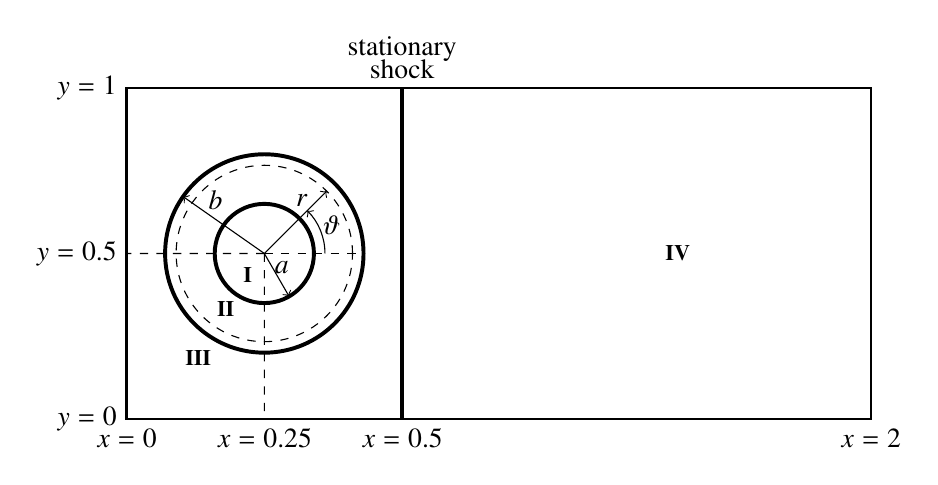
\begin{tikzpicture}[scale=7]
% Define angles for arrows
\def\angleA{-60}   % angle for radius a
\def\angleB{145}    % angle for radius b
\def\angleR{45}   % angle for radius r
% Radii
\def\rA{0.09}
\def\rB{0.18}
\def\rR{0.16}
\def\bottom{0.2}
\def\top{0.8}
% Circle center
\coordinate (C) at (0.25,0.5);
% Draw the outer rectangle
\draw[thick] (0,\bottom) rectangle (1.35,\top);
% Draw the shock line at x=0.5
\draw[very thick] (0.5,\bottom) -- (0.5,\top);
% Concentric circles with thicker lines for a and b
\draw[line width=0.5mm] (C) circle (\rA); % thicker circle for a
\draw[line width=0.5mm] (C) circle (\rB); % thicker circle for b
\draw[dashed] (C) circle (\rR);  % dashed circle for radius r
% Radius a arrow with centered label above
\draw[->] (C) -- ++({\angleA}:\rA)
node[pos=0.7, anchor=south] {\(a\)};
% Radius b arrow with centered label above
\draw[->] (C) -- ++({\angleB}:\rB)
node[pos=0.6, anchor=south] {\(b\)};
% Radius r arrow with centered label above
\draw[->] (C) -- ++({\angleR}:\rR)
node[pos=0.6, anchor=south] {\(r\)};
% Dashed projection lines to axes from center
\draw[dashed] (C) -- (0.25, \bottom); % vertical to x-axis
\draw[dashed] (C) -- (0, 0.5);  % horizontal to y-axis
% Axis labels
\node[anchor=east] at (0,\top) {$y=1$};
\node[anchor=east] at (0,\bottom) {$y=0$};
\node[anchor=north] at (0,\bottom) {$x=0$};
\node[anchor=north] at (0.5,\bottom) {$x=0.5$};
\node[anchor=north] at (1.35,\bottom) {$x=2$};
% Shock/stationary labels
\node[anchor=south] at (0.5,\top+0.03) {stationary};
\node[anchor=south] at (0.5,\top) {shock};
% Coordinate labels
\node[anchor=north] at (0.25,\bottom) {$x=0.25$};
\node[anchor=east] at (0,0.5) {$y=0.5$};
% Roman numerals for zones
\node[scale=0.8] at (0.22, 0.46) {\textbf{I}};
\node[scale=0.8] at (0.18, 0.4) {\textbf{II}};
\node[scale=0.8] at (0.13, 0.31) {\textbf{III}};
\node[scale=0.8] at (1.0, 0.5) {\textbf{IV}};
\draw[dashed] (0.25,0.5) -- (0.25+\rB,0.5); % horizontal dashed radius
% Define arc distance from center
\def\rTheta{0.11} % adjust this to move arc closer/farther from the center
% Theta angle arc and label
\draw[->] ($(C)+(\rTheta,0)$) arc[start angle=0, end angle=\angleR, radius=\rTheta];
\node at ($(C)+({\angleR/2}:1.2*\rTheta)$) {\(\vartheta\)};		
\end{tikzpicture}
\caption{\sf Example 7: Sketch of the simulation set-up.}
\label{fig48f}
\end{figure}

The velocity profile in vortex regions I and II is given, in terms of radial coordinates $(r,\vartheta)$ with respect to the center 
$(x_c,y_c)$:
$$
u(r,\vartheta)=u_{\rm III}-v_\vartheta\sin\vartheta,\quad v(r,\vartheta)=v_{\rm III}+v_\vartheta\cos{\vartheta},
$$
where 
$$
v_\vartheta:=\left\{\begin{aligned}
&v_m\,\frac{r}{a},&&r\le a,\\
&v_m\,\frac{a}{a^2-b^2}\left(r-\frac{b^2}{r}\right),&&a<r<b,\\
&0,&&r\ge b,\\
\end{aligned}\right.
$$
with $v_m:=M_v\sqrt{\gamma}$ being the the maximal angular velocity.

Density and pressure profiles inside the vortex are obtained imposing a balance between centripetal force and pressure gradients \cite{RCD},
resulting in
$$
p=p_{\rm III}\left(\frac{T}{T_{\rm III}}\right)^{\frac{\gamma}{\gamma-1}},\quad
\rho=\rho_{\rm III}\left(\frac{T}{T_{\rm III}}\right)^{\frac{1}{\gamma-1}},
$$
where $T_{\rm III}=\frac{p_{\rm III}}{\rho_{\rm III}R}$ is the constant temperature associated with the state of region III, with
$R=287$ J/kg-K being the specific gas constant of the fluid, and $T(r)$ is the temperature within the vortex:
$$
T(r)=\left\{\begin{aligned}
&A+\frac{\gamma-1}{R\gamma}\frac{v_m^2}{a^2}\frac{r^2}{2},&&r\le a,\\
&B+\frac{\gamma-1}{R\gamma}v_m^2\frac{a^2}{(a^2-b^2)^2}\left(\frac{r^2}{2}-2b^2\ln r-b^4\frac{r^{-2}}{2}\right),&&a<r<b,\\
&T_{\rm III},&&r\ge b,
\end{aligned}\right.
$$
where
$$
\begin{aligned}
B&=T_{\rm III}-\frac{\gamma-1}{R\gamma}v_m^2\frac{a^2}{(a^2-b^2)^2}\left(\frac{b^2}{2}-2b^2\ln b-b^4\frac{b^{-2}}{2}\right),\\[0.3ex]
A&=B+\frac{\gamma-1}{R\gamma}v_m^2\frac{a^2}{(a^2-b^2)^2}\left(\frac{a^2}{2}-2b^2\ln a-b^4\frac{a^{-2}}{2}\right)-
\frac{\gamma-1}{R\gamma}\frac{v_m^2}{2}.	
\end{aligned}
$$

Figure \ref{fig48} shows a Schlieren image of the numerical results displaying the magnitude of the density gradient field,
$\|\nabla\rho\|_2$, computed on a uniform mesh with $N_x=1200$ and $N_y=601$ at time $t=0.7$. In this figure, we have used the following
shading function:
$$
\exp{\left(-\frac{K\|\nabla\rho\|_2}{\max\|\nabla\rho\|_2}\right)},
$$
where the numerical density derivatives are computed using central differencing. The computed results agree well with those obtained in 
the literature.
\begin{figure}[ht!]
\centerline{\includegraphics[width=0.7\textwidth]{figure/shock_vortex_1200_601_schlieren_CFL0.25_SOLUTION_OCT_0000000.7000000.dat_hsv}}
\caption{\sf Example 7: Schlieren image of the density gradient.\label{fig48}}
\end{figure}

\section{Conclusions}\label{sec5}
In this paper, we have introduced a new active flux (AF) method for hyperbolic systems of conservation laws, for which we consider two
different formulations of the studied system (the original conservative formulation and a primitive one containing nonconservative
products), and discretize them on overlapping staggered meshes using two different numerical methods. Both the conservative and primitive
variables are evolved in time using second-order semi-discrete finite-volume (FV) methods. The nonconservative system is discretized by a
path-conservative central-upwind scheme and its solution is used to evaluate very simple numerical fluxes for the original conservative
system. The nonlinear stability of the resulting FV AF method is enforced with the help of a post-processing, which also guarantees a
conservative coupling between the two sets of variables. The performance of the proposed method has been demonstrated on a number of one-
and two-dimensional benchmarks.

We would like to emphasize that the main difficulty in designing higher-order extensions of the proposed FV AF method is related to
developing a high-order post-processing. Such post-processing should be based on a uniformly accurate reconstruction/interpolation. One can
use, for example, CWENO reconstructions/interpolations (see \cite{CPSV,CSV,SemVis} and references therein), and we plan to explore this
possibility in our future work.

We would also like to point out that having two sets of data for the discrete solution, which we evolve at each evolution step, has been
used to design a smoothness indicator based on the difference between these two solutions; see \cite{ChKuMi_proc}. This smoothness indicator
can be used to develop different adaptation strategies, which may substantially enhance the resolution achieved by the FV AF method.

\subsection*{Acknowledgment}
The work of A. Chertock was supported in part by NSF grant DMS-2208438. The work of A. Kurganov was supported in part by NSFC grants
12171226 and W2431004. The work of L. Micalizzi was supported in part by the LeRoy B. Martin, Jr. Distinguished Professorship Foundation.

\noindent \section*{In memoriam}

\noindent This paper is dedicated to the memory of Prof. Arturo Hidalgo L\'opez
($^*$July 03\textsuperscript{rd} 1966 - $\dagger$August 26\textsuperscript{th} 2024) of the Universidad Politecnica de Madrid, organizer of HONOM 2019 and active participant in many other editions of HONOM.
Our thoughts and wishes go to his wife Lourdes and his sister Mar\'ia Jes\'us, whom he left behind.


\bibliographystyle{siam}
\bibliography{sn-bibliography}
\end{document}
